\documentclass[10pt]{article}
\usepackage[margin=0.56in]{geometry}
\usepackage{booktabs,enumitem,fancyhdr,graphicx,overpic,tabularx,titlesec}
\usepackage[table]{xcolor}
\usepackage[hidelinks]{hyperref}
\graphicspath{{docs/lessons/assets/}{../assets/}}
\hypersetup{pdftitle={ADK Lesson 048: Kinetic Light Sculpture},
 pdfauthor={Kevin Shanahan},
 pdfsubject={Staged authorization, bounded logical motion, stop dominance, and exact light-intent mirroring},
 pdflang={en-US}}
\pagestyle{fancy}\fancyhf{}
\lhead{\textsc{ADK Lesson 048}}\rhead{Kinetic Light Sculpture}
\cfoot{\thepage}\setlength{\headheight}{14pt}
\setlength{\parindent}{0pt}\setlength{\parskip}{1.5pt}
\setlist{nosep,leftmargin=1.45em}
\titleformat{\section}{\Large\bfseries}{\thesection}{0.5em}{}
\titlespacing*{\section}{0pt}{7pt}{2pt}
\titlespacing*{\subsection}{0pt}{5pt}{2pt}
\newcommand{\lessonbox}[1]{\begin{center}\fbox{\parbox{0.92\linewidth}{#1}}\end{center}}
\newcommand{\blankline}{\rule{0.75in}{0.4pt}}

\begin{document}
\small
\begin{center}
 {\Huge\bfseries Kinetic Light Sculpture}\\[3pt]
 {\Large Authorize one bounded motif; mirror every logical step}\\[7pt]
 \fbox{\textbf{E0 COPIED REPLAY --- NO POWERED INPUT, LIGHT, OR MOTOR CLAIM}}
\end{center}
\begin{tabularx}{\linewidth}{@{}>{\bfseries}l X >{\bfseries}l X@{}}
Lesson & 048 --- project & Time & 140--200 minutes\\
Prerequisites & Lessons 046--047 & Board & compile-only Mega replay\\
Evidence & named memory result cells & Bounds & logical position \([-256,256]\)\\
\end{tabularx}

\lessonbox{\textbf{Project boundary.} This workbook composes copied tactile
and directional evidence with a pure logical step sequence and copied light
intent. It does not read a pin, energize an LED or coil, move a shaft, prove
position, qualify a driver, or provide a wiring plan.}

\section{Stage authorization before motion}
\begin{center}
% ADK visual: pencil
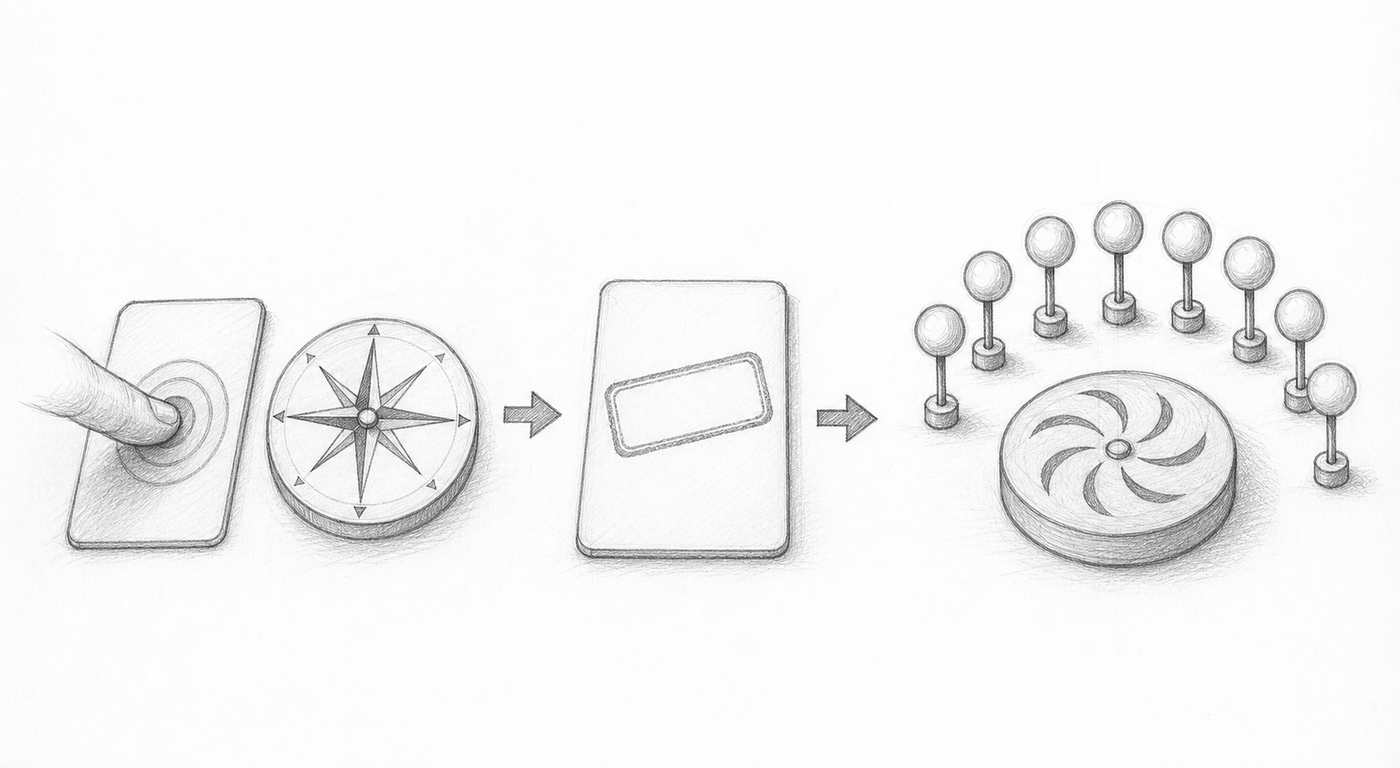
\includegraphics[width=0.97\linewidth,height=0.28\textheight,
 keepaspectratio]{048-staged-authorization-pencil.png}

\small\textit{Alternative text: a graphite-pencil sequence separates a
finger touch and eight-way direction, a retained pending authorization card,
and an inert imagined rotor beside eight lamps. Motion never begins in the
same frame that creates authorization.}
\end{center}

A valid touch event plus current directional evidence creates one
\texttt{Pending} authorization, even when its direction is Neutral. That
originating frame consumes no step and publishes no coil pattern. A healthy,
non-neutral, strictly forward frame may accept it as motion; Neutral, stop,
fault, expiry, or shutdown resolves it with the corresponding non-motion
outcome. For acceptance, the coordinator chooses one of eight fixed motifs,
asks the Lesson 047 sequencer to prepare it, verifies both prepared candidates,
and commits the transaction.

\begin{enumerate}
 \item \textbf{Acquire copied evidence:} one contact source, one directional
       source, one independent stop source, and one project frame identity.
 \item \textbf{Preview without mutation:} validate time, source domain,
       replay identity, age, skew, quality, and bounds.
 \item \textbf{Authorize once:} retain source identities, sequences,
       direction, originating frame, and \texttt{Pending} disposition.
 \item \textbf{Resolve later:} on the next healthy forward frame, accept one
       bounded non-neutral motif; Neutral resolves inhibited, while bounds,
       stop, fault, or expiry preserve their distinct terminal outcome.
\end{enumerate}

The resolving frame exposes the terminal authorization as
\texttt{Accepted}, \texttt{Inhibited}, or \texttt{BoundRejected}. The next
accepted forward frame clears that terminal record unless it replaces it with
a new resolution. Exact replay never authorizes twice.

\section{Map eight directions to fixed motifs}
\begin{tabularx}{\linewidth}{@{}l X r r@{}}
\toprule
Direction & logical direction & steps & interval\\
\midrule
North     & forward & 8  & 120 ms\\
NorthEast & forward & 12 & 100 ms\\
East      & forward & 16 & 80 ms\\
SouthEast & forward & 12 & 100 ms\\
South     & reverse & 8  & 120 ms\\
SouthWest & reverse & 12 & 100 ms\\
West      & reverse & 16 & 80 ms\\
NorthWest & reverse & 12 & 100 ms\\
\bottomrule
\end{tabularx}

These are project motifs, not physical angles or distances. The logical
position must remain inside \([-256,256]\). A request crossing either bound
becomes \texttt{BoundRejected}: no motion starts, no step is consumed, and
the travel-limit result cell becomes true. A fresh opposite authorization can
recover.

\newpage
\section{Mirror coil intent exactly}
On every accepted frame,
\[
\texttt{lights.shiftRegisterBits} =
\texttt{motion.coilIntent}.
\]
The equality is exact, including zero during authorization, cancellation,
stop, fault, expiry, and shutdown. The light record is copied semantic intent;
it is neither a shift-register driver nor evidence that a lamp was acquired.

\begin{tabularx}{\linewidth}{@{}l *{8}{>{\centering\arraybackslash}X}@{}}
\toprule
frame & 1 & 2 & 3 & 4 & 5 & 6 & 7 & 8\\
\midrule
coil byte & 01 & 03 & 02 & 06 & 04 & 0C & 08 & 09\\
light byte & 01 & 03 & 02 & 06 & 04 & 0C & 08 & 09\\
\bottomrule
\end{tabularx}

The row is one complete eight-frame logical sequence, not the direction-to-
motif table above. Reverse motion traverses the same configured frame order in
reverse. Because upper coil-intent bits are zero, upper light-byte bits are
also zero.

\begin{tabularx}{\linewidth}{@{}X X X X@{}}
\toprule
frame ID & coil intent & light bits & equal?\\
\midrule
\rule{0pt}{16pt}\blankline & \blankline & \blankline & \blankline\\[9pt]
\blankline & \blankline & \blankline & \blankline\\[9pt]
\blankline & \blankline & \blankline & \blankline\\
\bottomrule
\end{tabularx}

\section{Let stop dominate the transaction}
\begin{center}
% ADK visual: pencil
\begin{overpic}[width=0.90\linewidth]{048-stop-flow-pencil.png}
 \put(7,57){\scriptsize Inactive}
 \put(72,57){\scriptsize Ready}
 \put(75,27){\scriptsize Preview}
 \put(51,8){\scriptsize Running}
 \put(27,8){\scriptsize Complete}
 \put(6,28){\scriptsize Stopped}
 \put(43,54){\scriptsize\textbf{independent stop dominates}}
\end{overpic}

\small\textit{Alternative text: a rough pencil state loop contains inactive,
ready, preview, running, complete, and stopped cards, while a large hand is a
metaphor for copied independent-stop precedence. Fault is described in the
adjacent table; this is not a physical control layout.}
\end{center}

A valid active stop is assessed before malformed interaction evidence. It
cancels prepared or running motion, clears coil and light bits, inhibits a
pending authorization, and latches \texttt{Stopped}. A held stop cannot
restart. Release permits later healthy evidence to return to
\texttt{Ready}; release itself never creates authorization.

\begin{tabularx}{\linewidth}{@{}l X X@{}}
\toprule
Outcome & Required project result & Motion/light result\\
\midrule
\texttt{Ready} & healthy copied evidence; no pending motion & bits zero\\
\texttt{Preview} & pending authorization retained & steps and bits zero\\
\texttt{Running} & terminal \texttt{Accepted} on resolving frame & exact mirror\\
\texttt{Complete} & requested logical steps consumed & hold/off per policy\\
\texttt{Stopped} & valid independent stop dominates & coils and mirror zero\\
\texttt{Fault} & admitted source/motion failure latched & coils and mirror zero\\
\bottomrule
\end{tabularx}

\section{Distinguish rejection, stop, and fault}
Malformed frame identity, future time, ambiguous half-range order, changed
same-ID payload, impossible copied values, or unrecognized enum values reject
atomically. The prior project snapshot does not partially advance.

An admitted stop is not a fault. An admitted producer or sequence failure is
a fault and publishes a complete fault record with zero coil/light intent.
Fault is latched for the object lifetime; later healthy evidence and replay
cannot clear it. Recovery requires \texttt{shutdown()} followed by successful
\texttt{initialize()}. Shutdown returns \texttt{Inactive}, cancels motion,
publishes all-zero intent, and terminalizes a pending authorization as
\texttt{Inhibited}. That terminal record remains inspectable until successful
initialization clears the epoch.

\lessonbox{\textbf{Stop semantics at E0.} The copied stop record proves policy
precedence only. It is not an emergency-stop component, a safety-rated
function, or proof that physical power was independently removed.}

\section{Run the deterministic E0 workbook}
\begin{enumerate}
 \item Initialize. Predict \texttt{Ready}, logical position zero, no
       authorization, and all intent bits zero.
 \item Qualify a touch while supplying North. Predict \texttt{Pending} and
       zero requested steps in that frame. Repeat with Neutral: it still
       becomes pending, then resolves \texttt{Inhibited}.
 \item Supply a healthy forward frame. Predict \texttt{Accepted}, forward
       eight-step motion, 120 ms cadence, and exact coil/light equality.
 \item Repeat for all eight directions. Record the chosen direction, steps,
       cadence, and motif without claiming shaft motion or emitted light.
 \item Replay the resolving frame exactly. Predict no second motif. Supply one
       accepted forward frame and verify the terminal record clears.
 \item Collide an active valid stop with malformed directional evidence.
       Predict \texttt{Stopped}, pending disposition \texttt{Inhibited}, and
       all-zero intent.
 \item Drive copied logical position toward \(256\), then request a motif that
       would exceed it. Predict a bound rejection, travel-limit intent,
       and no step. Repeat at \(-256\).
 \item Inject source failure, command expiry, timing rollover, and shutdown.
       Predict fault-safe or inactive all-zero intent without partial state.
\end{enumerate}

\subsection*{E0 result cells}
\begin{tabularx}{\linewidth}{@{}X X X X X@{}}
\toprule
frame & phase & authorization & position & status\\
\midrule
\rule{0pt}{16pt}\blankline & \blankline & \blankline & \blankline & \blankline\\[9pt]
\blankline & \blankline & \blankline & \blankline & \blankline\\[9pt]
\blankline & \blankline & \blankline & \blankline & \blankline\\
\bottomrule
\end{tabularx}

\begin{tabularx}{\linewidth}{@{}X X X X X@{}}
\toprule
direction & steps & coil bits & light bits & stop/limit\\
\midrule
\rule{0pt}{16pt}\blankline & \blankline & \blankline & \blankline & \blankline\\[9pt]
\blankline & \blankline & \blankline & \blankline & \blankline\\[9pt]
\blankline & \blankline & \blankline & \blankline & \blankline\\
\bottomrule
\end{tabularx}

\section{Interpret only what E0 observes}
\textbf{Acquisition prediction.} Recognized nonzero source identities,
forward-or-repeat chronology, bounded age/skew, and self-consistent copied
contact, direction, and stop records form one admissible frame.

\textbf{Acquisition observation.} Inspect \texttt{frameId}, copied source
identities, sequences, ages, qualities, project status, and accepted
authorization records in host memory.

\textbf{Acquisition interpretation.} Acceptance proves the pure copied-data
contract. It does not prove a touch board, joystick, stop switch, clock, pin,
or electrical endpoint was acquired.

\textbf{Safe-state prediction.} Stop, fault, expiry, bound rejection, and
shutdown publish the specified terminal disposition and zero motion/light
intent where required.

\textbf{Safe-state observation.} Inspect phase, motion disposition, coil
intent, light byte, pending/terminal records, travel-limit flag, and status.

\textbf{Safe-state interpretation.} An all-zero memory record proves only the
E0 policy result. It does not prove de-energized coils, dark LEDs, stationary
hardware, or removed motor power.

\section{Bound the compile-only composition}
The canonical Mega replay uses fixed storage and no heap, live input GPIO,
stepper driver, shift-register endpoint, motor supply, timer-owned motion, or
hardware debugger. Its final measured package size is:

\begin{tabularx}{\linewidth}{@{}X r r@{}}
\toprule
Artifact & measured & budget\\
\midrule
Mega flash & 22,216 bytes & 28,672 bytes\\
static SRAM & 1,470 bytes & 2,048 bytes\\
\texttt{KineticLightSculpture} object & 502 bytes & 512 / 640 bytes\\
static compiler/link stack plus timer-0 ISR & 687 bytes & evidence only\\
SRAM remaining after static and stack/ISR & 6,035 bytes & 1,024-byte margin\\
\bottomrule
\end{tabularx}

The 687-byte estimate is conservative static compiler/link evidence, not
runtime high-water. Compilation is packaging evidence, not runtime stack,
current, timing, temperature, motion, or electrical shutdown evidence.

\section{Leave E1 input and light acceptance blank}
\lessonbox{\textbf{E1 remains open.} E1 may qualify exact low-energy tactile,
directional, stop, and indicator specimens. It still may not energize a
stepper coil or moving load.}

\begin{tabularx}{\linewidth}{@{}>{\bfseries}l X@{}}
Exact specimen and revision markings & \rule{0pt}{16pt}\hrulefill\\[9pt]
Primary datasheet sources & \hrulefill\\[9pt]
Supply, logic levels, and pin order & \hrulefill\\[9pt]
Input qualification and active polarity & \hrulefill\\[9pt]
Indicator resistors and measured current & \hrulefill\\[9pt]
Independent stop observation & \hrulefill\\[9pt]
Electrical rollback observation & \hrulefill\\[9pt]
Reviewer, date, acceptance record & \hrulefill\\
\end{tabularx}

\newpage
\section{Leave E2 motion acceptance blank}
\lessonbox{\textbf{E2 remains open.} A likely 28BYJ-48 label and ULN2003
carrier do not establish motor voltage, winding, driver topology, clamp
connection, safe current, or motion. No physical build is authorized here.}

\begin{tabularx}{\linewidth}{@{}>{\bfseries}l X@{}}
Exact motor, winding, and driver identity & \rule{0pt}{16pt}\hrulefill\\[9pt]
Electrically authoritative schematic review & \hrulefill\\[9pt]
Separate current-limited supply and common & \hrulefill\\[9pt]
Measured coil and aggregate current & \hrulefill\\[9pt]
Thermal, cadence, and restraint evidence & \hrulefill\\[9pt]
Measured travel and bound behavior & \hrulefill\\[9pt]
Independent power-removal safe state & \hrulefill\\[9pt]
Reviewer, date, acceptance record & \hrulefill\\
\end{tabularx}

Future E2 work must use a lightweight, stable tabletop mechanism with guarded
pinch points, no loose load, no sharp or high-inertia feature, no stored
energy, and a stop/power-removal path independent of software. This project
never controls a launcher, vehicle, door lock, lifting mechanism, or safety
device.

\section{Software evidence and further work}
Deterministic tests cover initialization, all eight motifs, staged and replayed
authorization, terminal-record lifetime, transaction rollback, source-domain
changes, stop dominance and release, expiry, bounds, fault reinitialization, rollover,
storage lifetime, light equality, and shutdown.

\begin{itemize}
 \item \href{https://github.com/spincyc/adk/blob/main/examples/Lesson048KineticLightSculpture/Lesson048KineticLightSculpture.ino}
       {Canonical compile-only Lesson 048 sketch}.
 \item \href{https://github.com/spincyc/adk/blob/main/tests/test_kinetic_sculpture.cpp}
       {Deterministic kinetic-sculpture tests}.
 \item \href{https://github.com/spincyc/adk/blob/main/src/kinetic_sculpture.h}
       {Kinetic-sculpture interface}.
 \item \href{https://github.com/spincyc/adk/blob/main/docs/design/LESSONS_046_048_KINETIC_SCULPTURE_PLAN.md}
       {Lessons 046--048 design record}.
 \item \href{https://github.com/spincyc/adk/blob/main/docs/TESTING.md}
       {Deterministic testing contract}.
 \item \href{https://github.com/spincyc/adk/blob/main/docs/SAFETY_MODEL.md}
       {Safety model}.
\end{itemize}

This untagged print edition has a searchable HTML alternative.
It makes no PDF/UA or physical accessibility claim.
\end{document}
